\newpage
\section*{IMPLEMENTATION}
\addcontentsline{toc}{section}{IMPLEMENTATION}

\subsection*{Double Side Band -- Full Carrier (DSB-FC)}
\phantomsection
\addcontentsline{toc}{subsection}{DSB-FC}
The DSB-FC signal is implemented by varying the amplitude of a high-frequency carrier in
proportion to the message signal. In the implementation, a low-frequency sinusoidal message
signal is generated and added to a constant carrier term to ensure that the carrier is
transmitted in full. The resulting signal contains the carrier component along with both
upper and lower sidebands.

\begin{enumerate}[itemsep=6pt, parsep=4pt, leftmargin=*, label={\textbf{\arabic*.}}]

\item \textbf{Sampling frequency (Fs)} \\
Determines how finely the signal is sampled. Must satisfy Nyquist: $Fs > 2 \, f_m$.  
Effect: higher Fs gives smoother signal and more accurate frequency spectrum.

\item \textbf{Duration (T)} \\
Total time of the signal.  
Effect: longer T improves frequency resolution in FFT.

\item\textbf{ Message amplitude (Am)} \\
Amplitude of the baseband signal.  
Effect: larger Am increases envelope height; if too large, over-modulation occurs.

\item \textbf{Carrier amplitude (Ac)} \\
Amplitude of the high-frequency carrier.  
Effect: higher Ac produces stronger signal and ensures envelope detection works. Typically, $Ac > Am$.

\item \textbf{Message frequency (fm)} \\
Frequency of the baseband signal.  
Effect: higher fm → faster envelope changes; bandwidth = $2 f_m$.

\item \textbf{Carrier frequency (fc)} \\
Frequency of the carrier, must be much higher than fm.  
Effect: shifts signal in frequency domain; envelope shape unchanged.

\item \textbf{Modulation index / amplitude sensitivity (ka)} \\
Scales the message relative to the carrier.  
Effect: higher ka strengthens modulation; ka $> 1$ can cause over-modulation.

\end{enumerate}

\newpage
\subsubsection*{Code:}

\begin{minted}[linenos, fontsize=\small]{python}
import numpy as np
import matplotlib.pyplot as plt

# Defining Sampling Parameters
Fs = 10000                 # Sampling frequency (Hz)
T = 0.01                   # Duration of signal (seconds)
t = np.arange(0, T, 1/Fs)  # Time vector (sampling instances)
ka = 1                     # amplitude sensitivity

# Fs must satisfy Nyquist: Fs > 2*fm

# Baseband Signal (Message Signal)
# Single-tone baseband signal m(t) = Am*cos(2*pi*fm*t)
Am = 1                     # Amplitude of message signal
fm = 50                    # Frequency of message signal (Hz)
m_t = Am * np.sin(2 * np.pi * fm * t)

# Carrier Signal (High-frequency carrier)
Ac = 5                     # Carrier amplitude
fc = 1000                  # Carrier frequency (Hz)
c_t = Ac * np.cos(2 * np.pi * fc * t)

# DSB-FC Modulation (The carrier is transmitted in full)
# Formula: s(t) = Ac * [1 + ka * m(t)] * cos(2*pi*fc*t)
s_dsbfc = Ac * (1 + ka * m_t) * np.cos(2 * np.pi * fc * t)

# Ploting Time-Domain Signals
plt.figure(figsize=(12, 8))

plt.subplot(3,1,1)
plt.plot(t, m_t, 'b', linewidth=1.5)
plt.title('Message Signal m(t)')
plt.xlabel('Time [s]')
plt.ylabel('Amplitude')
plt.grid(True)

plt.subplot(3,1,2)
plt.plot(t, c_t, 'r', linewidth=1.5)
plt.title('Carrier Signal c(t)')
plt.xlabel('Time [s]')
plt.ylabel('Amplitude')
plt.grid(True)

plt.subplot(3,1,3)
plt.plot(t, s_dsbfc, 'g', linewidth=1.5)
plt.title('DSB-FC Modulated Signal s(t)')
plt.xlabel('Time [s]')
plt.ylabel('Amplitude')
plt.grid(True)

plt.tight_layout()
plt.show()

# Frequency-Domain Analysis
N = len(s_dsbfc)
S_f = np.fft.fft(s_dsbfc)/N       # FFT and normalization
f = np.fft.fftfreq(N, 1/Fs)       # Frequency axis 

f_pos = f[:N//2]                  # Take only positive frequencies
S_f_pos = 2 * np.abs(S_f[:N//2])  # Multiply by 2 to account for symmetry

plt.figure(figsize=(10,4))
plt.plot(f_pos, S_f_pos, 'm', linewidth=1.5)
plt.title("Magnitude Spectrum of DSB-FC Signal")
plt.xlabel("Frequency [Hz]")
plt.ylabel("Magnitude")
plt.grid(True)
plt.show()
\end{minted}

\subsubsection*{Output:}
The above plots are obtained using the following parameters: 
sampling frequency $Fs = 10$ kHz, signal duration $T = 0.01$s, 
message amplitude $A_m = 1$, carrier amplitude $A_c = 5$, 
message frequency $f_m = 50$ Hz, carrier frequency $f_c = 1000$ Hz, 
and modulation index $k_a = 1$.

\begin{figure}[!ht]
    \centering
    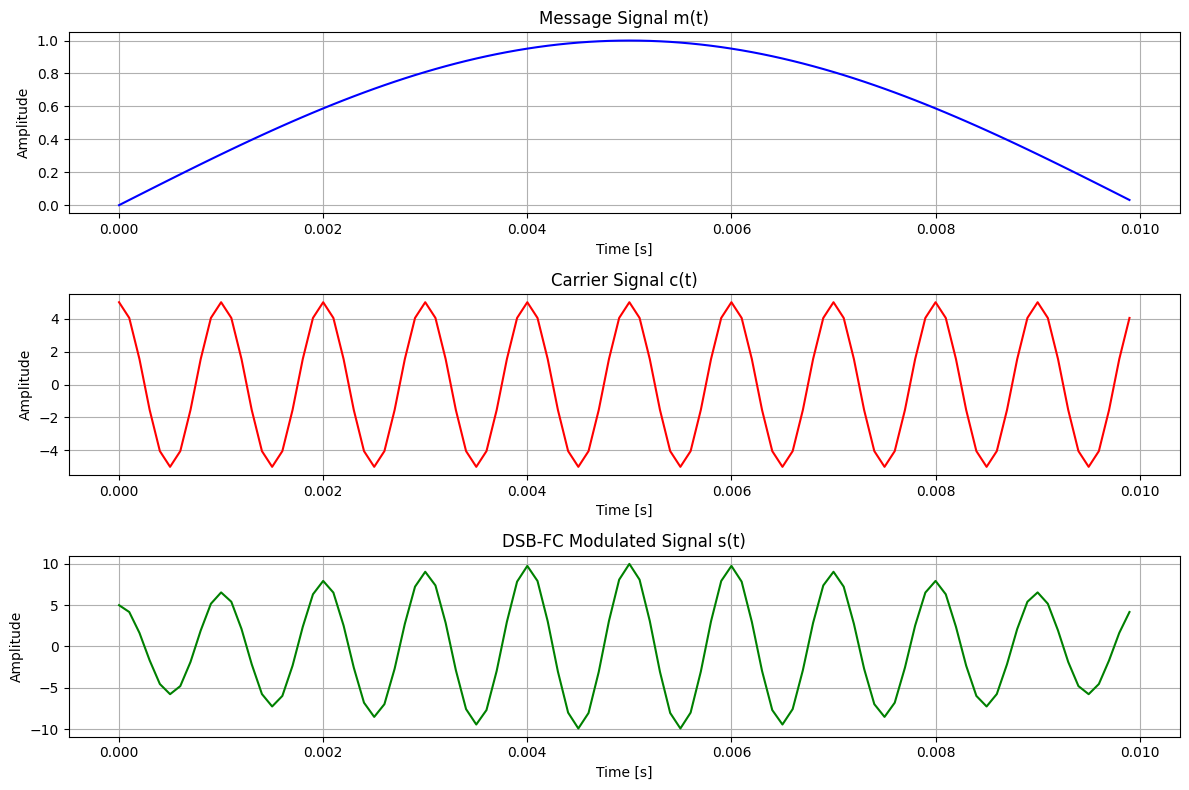
\includegraphics[width=0.9\textwidth]{images/output1.png} 
    \caption{Plots of (a) Message Signal, (b) Carrier Signal, and (c) DSB-FC Modulated Signal}
    \label{fig:output1}
\end{figure}
\begin{figure}[!ht]
    \centering
    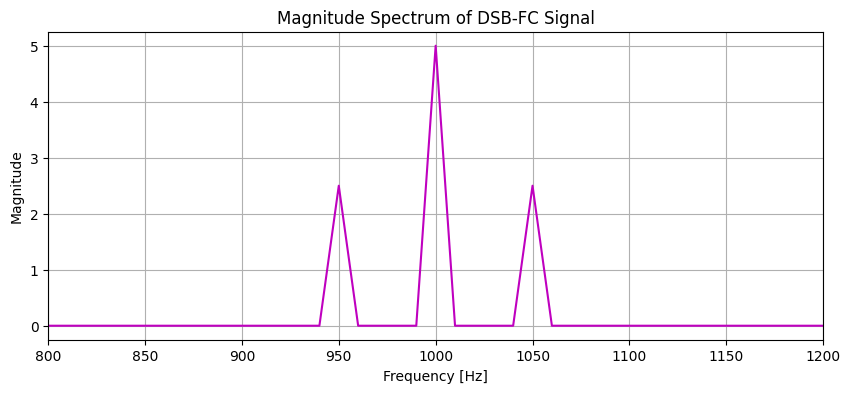
\includegraphics[width=0.9\textwidth]{images/output2.png} 
    \caption{Plots of DSB-FC spectrum}
    \label{fig:output2}
\end{figure}


\subsubsection*{Observations:}

From the time-domain plot (Figure~\ref{fig:output1}):
\begin{itemize}[itemsep=4pt, parsep=2pt]
    \item The message signal $m(t)$ is a low-frequency sinusoid.
    \item The carrier signal $c(t)$ is a high-frequency cosine wave.
    \item The DSB-FC modulated signal $s(t)$ shows that the amplitude of the carrier varies according to the message signal, forming an envelope that matches $m(t)$.
\end{itemize}

From the frequency-domain plot (Figure~\ref{fig:output2}):
\begin{itemize}[itemsep=4pt, parsep=2pt]
    \item The spectrum shows a peak at the carrier frequency $f_c = 1000$ Hz.
    \item Two sidebands appear at $f_c \pm f_m$ (i.e., 950 Hz and 1050 Hz), carrying the message information.
    \item The bandwidth of the DSB-FC signal is $2 f_m = 100$ Hz.
\end{itemize}


\subsubsection*{Variations of Different Parameters:}

\begin{figure}[!ht]
    \centering
    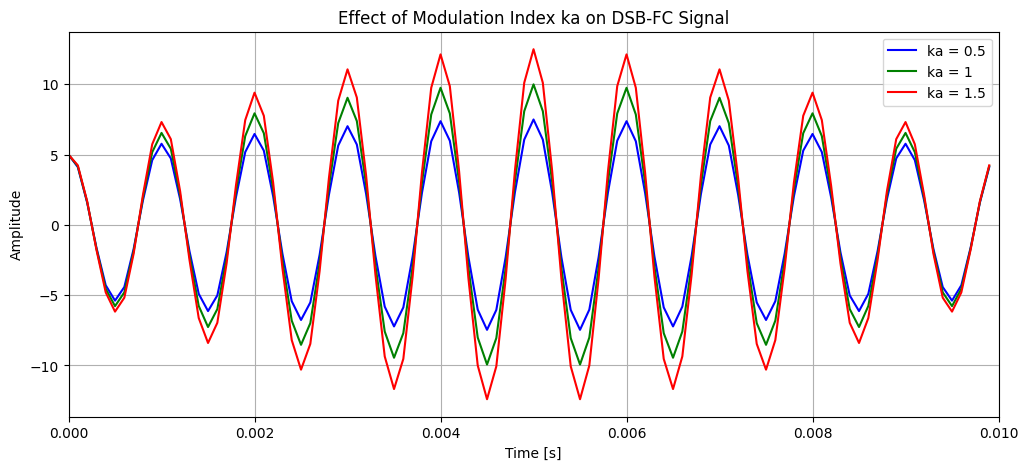
\includegraphics[width=0.9\textwidth]{images/ka_variation.png}
    \caption{Effect of modulation index $k_a$ on DSB-FC signal}
    \label{fig:ka_variation}
\end{figure}

\begin{figure}[!ht]
    \centering
    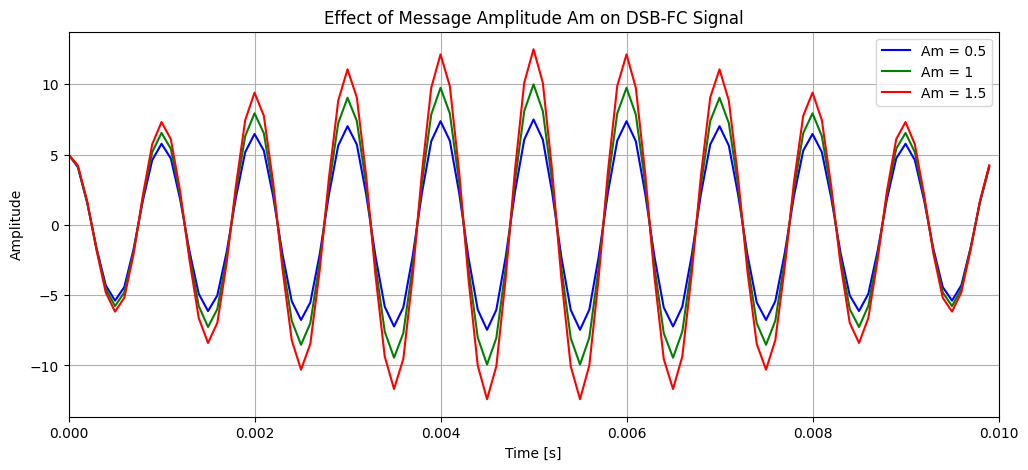
\includegraphics[width=0.9\textwidth]{images/Am_variation.png}
    \caption{Effect of message amplitude $A_m$ on DSB-FC signal}
    \label{fig:Am_variation}
\end{figure}

\begin{figure}[!ht]
    \centering
    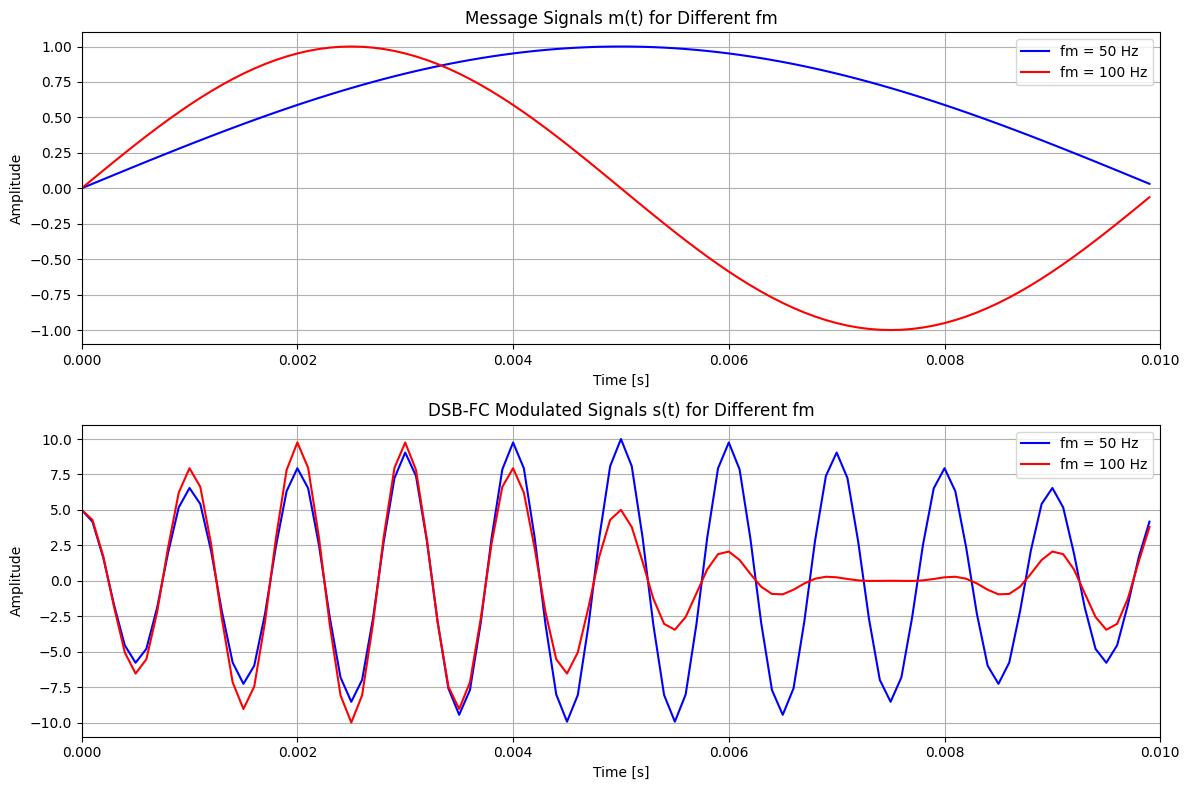
\includegraphics[width=0.9\textwidth]{images/fm_time_variation.png}
    \caption{Effect of message frequency $f_m$ on DSB-FC signal in time domain}
    \label{fig:fm_time}
\end{figure}

\begin{figure}[!ht]
    \centering
    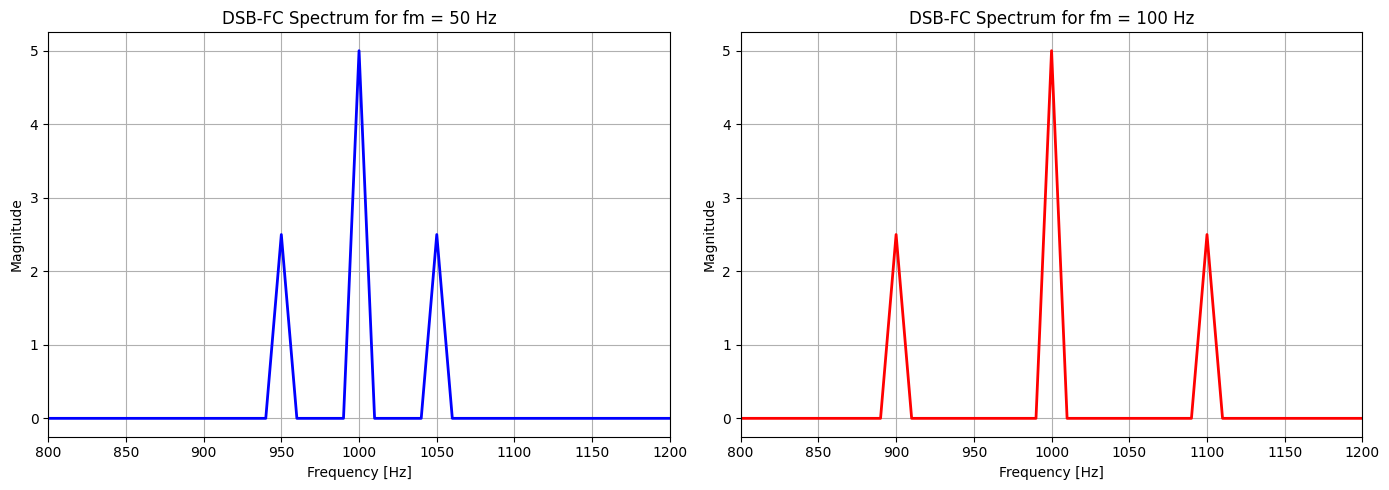
\includegraphics[width=0.9\textwidth]{images/fm_freq_variation.png}
    \caption{Effect of message frequency $f_m$ on DSB-FC spectrum} 
    \label{fig:fm_freq}
\end{figure}

\begin{itemize}[itemsep=2pt]
    \item DSB-FC spectrum shows a strong carrier peak at $f_c$ and two smaller sidebands at $f_c \pm f_m$. 
    \item fm = 50 Hz: envelope oscillates slowly; sidebands at 950 Hz and 1050 Hz, bandwidth = 100 Hz.
    \item fm = 100 Hz: envelope oscillates faster; sidebands at 900 Hz and 1100 Hz, bandwidth = 200 Hz.
    \item Higher message frequency increases both the envelope oscillation rate and the spectrum bandwidth.
\end{itemize}
